\chapter{RBFNN-based identification on a simple network}
\label{NN_based_example}

\emph{In this part of the appendix, a numerical example of system identification is carried out on a simple network.}

\section{The EPANET model}
\label{example1_EPANET}

The reason for testing the identification method on data from a simple EPANET model is that, in simulation, several different operations of the network can be studied. On a real world network, typically the system cannot be operated arbitrarily. Therefore, the network shown in \figref{fig:epanet_example1_id} has been created to mimic the behaviour of a multi-inlet, single-WT system. 

%EPANET example network for identification
\begin{figure}[H]
\centering
%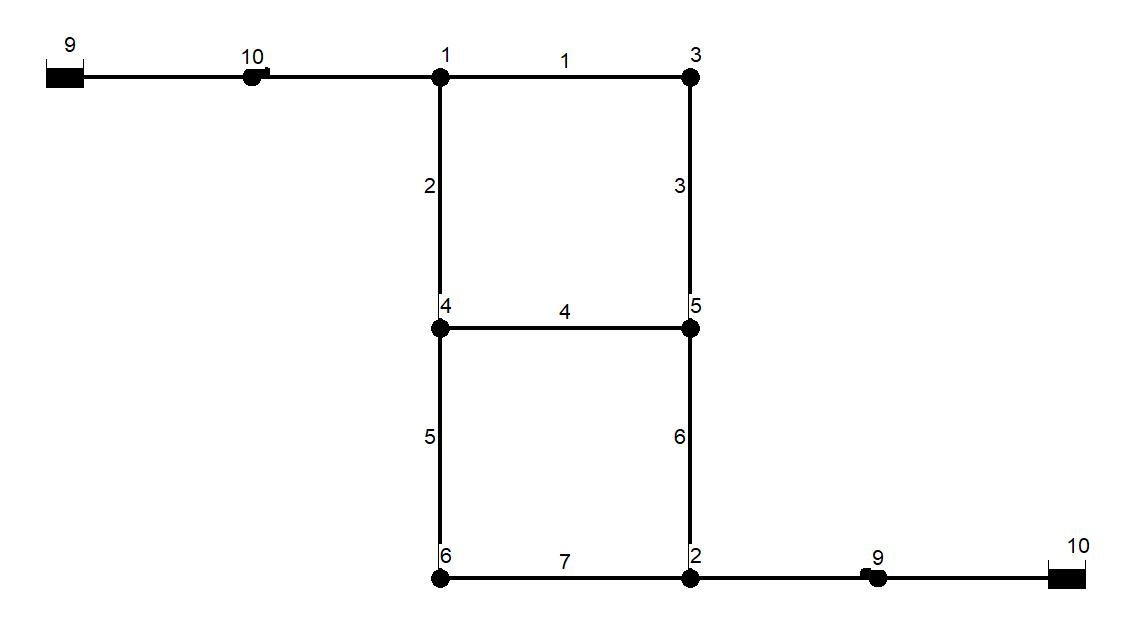
\includegraphics[width=0.6\textwidth]{report/pictures/example1_epanetmodel}
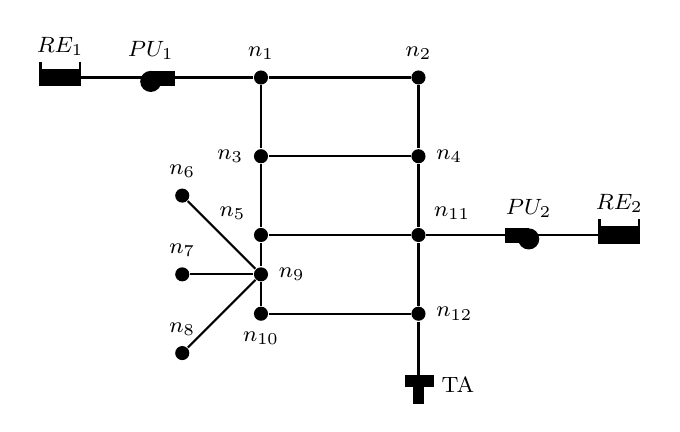
\begin{tikzpicture}[semithick,state/.style ={ draw,shape=circle,scale=0.9}]

\node[circle,fill,inner sep=1.8pt,label=above : \footnotesize$n_1$] (A) at (0,0) {};
\node[circle,fill,inner sep=1.8pt,label=above : \footnotesize$n_2$] (B) at (2,0) {};
\node[circle,fill,inner sep=1.8pt,label= left: \footnotesize$n_3$] (C) at (0,-1) {};
\node[circle,fill,inner sep=1.8pt,label= right: \footnotesize$n_4$] (D) at (2,-1) {};
\node[circle,fill,inner sep=1.8pt,label= above right: \footnotesize $n_{11}$] (E) at (2,-2) {};
\node[circle,fill,inner sep=1.8pt,label= above left: \footnotesize$n_5$] (F) at (0,-2) {};
\node[circle,fill,inner sep=1.8pt,label= below : \footnotesize$n_{10}$] (G) at (0,-3) {};
\node[circle,fill,inner sep=1.8pt,label=  right: \footnotesize$n_9$] (H) at (0,-2.5) {};
\node[circle,fill,inner sep=1.8pt,label=  right: \footnotesize$n_{12}$] (I) at (2,-3) {};
\node[circle,fill,inner sep=1.8pt,label=  above: \footnotesize$n_6$] (J) at (-1,-1.5) {};
\node[circle,fill,inner sep=1.8pt,label=  above: \footnotesize $n_7$] (M) at (-1,-2.5) {};
\node[circle,fill,inner sep=1.8pt,label=  above: \footnotesize $n_8$] (L) at (-1,-3.5) {};



\draw [thick] (A) --  (B) node[above  =0.05 cm] {\footnotesize$$};
\path (A) edge [thick]  node[left  =0.05 cm] {\footnotesize$$} (C);
\path (B) edge [thick] node[right  =0.05 cm] {\footnotesize$$} (D);
\path (C) edge [thick] node[above  =0.05 cm] {\footnotesize$$} (D);
\path (C) edge [thick] node[left  =0.05 cm] {\footnotesize$$} (F);
\path (D) edge [thick] node[right  =0.05 cm] {\footnotesize$$} (E);
\path (E) edge [thick] node[below  =0.05 cm] {\footnotesize$$} (F);
\path (F) edge [thick] node[below  =0.05 cm] {\footnotesize$$} (H);
\path (H) edge [thick] node[below  =0.05 cm] {\footnotesize$$} (G);
\path (H) edge [thick] node[below  =0.05 cm] {\footnotesize$$} (J);
\path (H) edge [thick] node[below  =0.05 cm] {\footnotesize$$} (M);
\path (H) edge [thick] node[below  =0.05 cm] {\footnotesize$$} (L);
\path (G) edge [thick] node[below  =0.05 cm] {\footnotesize$$} (I);
\path (E) edge [thick] node[below  =0.05 cm] {\footnotesize$$} (I);

%PU2
\node[circle,fill,inner sep=2.7pt,label= above : \footnotesize $ PU_2$] (I) at (3.4,-2.05) {};
\draw [thin,fill] (3.1,-1.92) rectangle (3.4,-2.1);


\begin{scope}[xscale=-1,yscale=1]
%PU1
\node[circle,fill,inner sep=2.7pt,label= above : \footnotesize $ PU_1$] (I) at (3.4-2,-2.05+2) {};
\draw [thin,fill] (3.1-2,-1.92+2) rectangle (3.4-2,-2.1+2);

\end{scope}

\draw [thick](2.1,-2) -- (3.1,-2);
\draw [thick, fill] (1.84,-3.79) rectangle (2.18,-3.92);
\draw [thick,fill] (1.95,-3.92) rectangle (2.06,-4.13);
\draw [thick](2,-3.1) -- (2,-3.8);
\node at (2.5,-3.9) {\footnotesize TA};


\draw [thick](-0.1,0) -- (-1.1,0);


\draw [thick](3.5,-2) -- (4.3,-2);
\draw [thick](-1.5,0) -- (-2.3,0);
\draw [thick](-2.3,0.2) -- (-2.3,-0.1) -- (-2.8,-0.1) -- (-2.8,0.2);
\draw [thick,fill] (-2.8,0.1) rectangle (-2.3,-0.1);
\draw [thick](4.3,-1.8) -- (4.3,-2.1) -- (4.8,-2.1) -- (4.8,-1.8);
\draw [thick,fill] (4.3,-1.9) rectangle (4.8,-2.1);
\node at (-2.55,0.4) {\footnotesize $RE_1$};
\node at (4.55,-1.6) {\footnotesize $RE_2$};
\end{tikzpicture} 
\caption{Multi-inlet, Single-WT example network.}
\label{fig:epanet_example1_id}
\end{figure}
\vspace{-3mm}

The network shown in \figref{fig:epanet_example1_id} consists of two pumping stations $PU_1$ and $PU_2$ and a Water Tank $TA$. Furthermore, in EPANET reservoirs are required for operating the pumps. The reservoirs $RE_1$ and $RE_2$ are different from WTs in a sense that they cannot be emptied in the simulation. Additionally, the physical properties of the network can be found in \appref{physical_properties_example1}. 

The controls implemented on the network are based on simple time scheduling of the two pumping stations. Both pumps turn off when the pressure head is above $19.85 [m]$ in the WT. $PU_2$ turns on again if the pressure head in the WT decreases to $19.55 [m]$. Furthermore, $PU_2$ turns on again only if the pressure head delivered by $PU_1$ exceeds $43 [m]$. The initial pressure head in the WT is $19.5 [m]$.

\section{NN based identification on an example network1}
\label{NN_based_example1} 

\newpage


  %Inlet flow1
 \begin{figure}[h!]
 \centering
 %\hspace{0mm}
 %
\includegraphics[width=0.35\textwidth]{report/pictures/missingfigure}
 % This file was created by matlab2tikz.
%
%The latest updates can be retrieved from
%  http://www.mathworks.com/matlabcentral/fileexchange/22022-matlab2tikz-matlab2tikz
%where you can also make suggestions and rate matlab2tikz.
%
\definecolor{mycolor1}{rgb}{0.00000,0.44700,0.74100}%
%
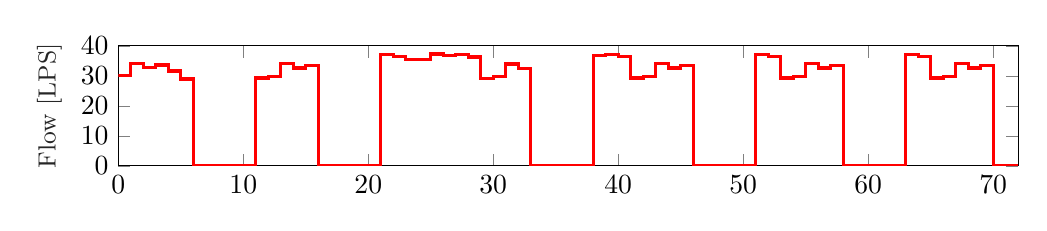
\begin{tikzpicture}

\begin{axis}[%
width=4.5in,
height=0.6in,
at={(0.948in,2.263in)},
scale only axis,
xmin=0,
xmax=72,
%xlabel style={font=\color{white!15!black}},
%xlabel={Time [h]},
ymin=0,
ymax=40,
ylabel style={font=\color{white!15!black}},
ylabel={\small Flow [LPS]},
axis background/.style={fill=white},
%title style={font=\bfseries},
%title={Inlet flows $\bar{d}_{\mathcal{K},1}$ and $\bar{d}_{\mathcal{K},2}$}
]
\addplot[const plot, color=red, line width=1.2pt, forget plot] table[row sep=crcr] {%
0	30.0046\\
1	34.1741\\
2	32.762\\
3	33.6315\\
4	31.5564\\
5	28.9859\\
6	0\\
7	0\\
8	0\\
9	0\\
10	0\\
11	29.2774\\
12	29.842\\
13	34.0029\\
14	32.5962\\
15	33.462\\
16	0\\
17	0\\
18	0\\
19	0\\
20	0\\
21	37.1075\\
22	36.3696\\
23	35.4455\\
24	35.4014\\
25	37.2252\\
26	36.6992\\
27	37.025\\
28	36.2878\\
29	29.2108\\
30	29.7754\\
31	33.9328\\
32	32.5282\\
33	0\\
34	0\\
35	0\\
36	0\\
37	0\\
38	36.7844\\
39	37.1088\\
40	36.371\\
41	29.2785\\
42	29.8431\\
43	34.0041\\
44	32.5973\\
45	33.4631\\
46	0\\
47	0\\
48	0\\
49	0\\
50	0\\
51	37.1071\\
52	36.3693\\
53	29.2771\\
54	29.8417\\
55	34.0026\\
56	32.5959\\
57	33.4617\\
58	0\\
59	0\\
60	0\\
61	0\\
62	0\\
63	37.1075\\
64	36.3696\\
65	29.2774\\
66	29.842\\
67	34.0029\\
68	32.5962\\
69	33.4619\\
70	0\\
71	0\\
72	0\\
};

\end{axis}
\end{tikzpicture}% 
 %\vspace{-1.5mm}
 %\caption{}
 \label{fig:inlet_flows_example1}
 \end{figure}

\vspace{-8mm}

   %Inlet flow2
 \begin{figure}[h!]
 \centering
 \hspace{0.15mm}
 %
\includegraphics[width=0.35\textwidth]{report/pictures/missingfigure}
 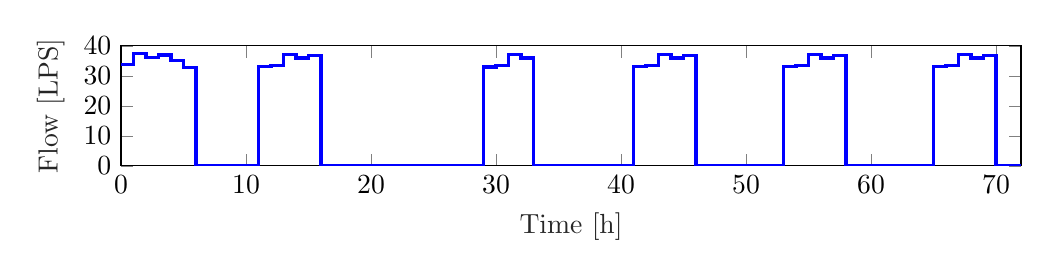
\begin{tikzpicture}
\begin{axis}[%
width=4.5in,
height=0.6in,
at={(0.948in,0.521in)},
scale only axis,
xmin=0,
xmax=72,
xlabel style={font=\color{white!15!black}},
xlabel={Time [h]},
ymin=0,
ymax=40,
ylabel style={font=\color{white!15!black}},
ylabel={Flow  [LPS]},
axis background/.style={fill=white},
%title style={font=\bfseries},
%title={Inlet flow - $\bar{d}_{\mathcal{K},2}$}
]
\addplot[const plot, color=blue, line width=1.2pt, forget plot] table[row sep=crcr] {%
0	33.6848\\
1	37.3894\\
2	36.1246\\
3	36.8904\\
4	35.0355\\
5	32.7372\\
6	0\\
7	0\\
8	0\\
9	0\\
10	0\\
11	33.0295\\
12	33.5214\\
13	37.2163\\
14	35.9569\\
15	36.7191\\
16	0\\
17	0\\
18	0\\
19	0\\
20	0\\
21	0\\
22	0\\
23	0\\
24	0\\
25	0\\
26	0\\
27	0\\
28	0\\
29	32.9627\\
30	33.4544\\
31	37.1454\\
32	35.8883\\
33	0\\
34	0\\
35	0\\
36	0\\
37	0\\
38	0\\
39	0\\
40	0\\
41	33.0306\\
42	33.5225\\
43	37.2175\\
44	35.9581\\
45	36.7203\\
46	0\\
47	0\\
48	0\\
49	0\\
50	0\\
51	0\\
52	0\\
53	33.0292\\
54	33.5211\\
55	37.216\\
56	35.9566\\
57	36.7188\\
58	0\\
59	0\\
60	0\\
61	0\\
62	0\\
63	0\\
64	0\\
65	33.0295\\
66	33.5214\\
67	37.2163\\
68	35.9569\\
69	36.7191\\
70	0\\
71	0\\
72	0\\
};
%\addlegendentry{\tiny $\bar{d}_{\mathcal{K},2}$ }
\end{axis}
\end{tikzpicture} 
 \vspace{-1.5mm}
 \caption{Inlet flows of the two pumping stations PU1 and PU2.}
 \label{fig:inlet_flows_example1}
 \end{figure}

 

\vspace{-3mm}

   %WT head
 \begin{figure}[H]
 \centering
 %
\includegraphics[width=0.35\textwidth]{report/pictures/missingfigure}
 % This file was created by matlab2tikz.
%
%The latest updates can be retrieved from
%  http://www.mathworks.com/matlabcentral/fileexchange/22022-matlab2tikz-matlab2tikz
%where you can also make suggestions and rate matlab2tikz.
%
\definecolor{mycolor1}{rgb}{0.00000,0.44700,0.74100}%
%
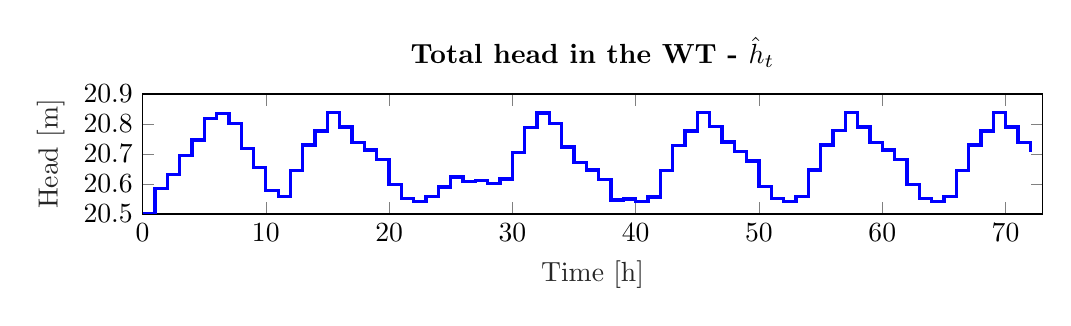
\begin{tikzpicture}

\begin{axis}[%
width=4.5in,
height=0.6in,
at={(0.761in,0.425in)},
scale only axis,
xmin=0,
xmax=73,
xlabel style={font=\color{white!15!black}},
xlabel={Time [h]},
ymin=20.5,
ymax=20.9,
ylabel style={font=\color{white!15!black}},
ylabel={Head  [m]},
axis background/.style={fill=white},
title style={font=\bfseries},
title={Total head in the WT - $\hat{h}_{t}$}
]
\addplot[const plot, color=blue, line width=1.2pt, forget plot] table[row sep=crcr] {%
0	20.5\\
1	20.5847\\
2	20.6325\\
3	20.6946\\
4	20.7469\\
5	20.8177\\
6	20.8338\\
7	20.8017\\
8	20.7183\\
9	20.6541\\
10	20.5771\\
11	20.5572\\
12	20.6458\\
13	20.7299\\
14	20.777\\
15	20.8386\\
16	20.79\\
17	20.7387\\
18	20.713\\
19	20.681\\
20	20.5975\\
21	20.5508\\
22	20.5419\\
23	20.5572\\
24	20.5901\\
25	20.6229\\
26	20.6078\\
27	20.6109\\
28	20.6018\\
29	20.617\\
30	20.7053\\
31	20.7891\\
32	20.836\\
33	20.8005\\
34	20.7235\\
35	20.6721\\
36	20.6465\\
37	20.6144\\
38	20.5466\\
39	20.5498\\
40	20.5409\\
41	20.5562\\
42	20.6448\\
43	20.7289\\
44	20.776\\
45	20.8376\\
46	20.7915\\
47	20.7402\\
48	20.7081\\
49	20.676\\
50	20.5926\\
51	20.5511\\
52	20.5421\\
53	20.5575\\
54	20.646\\
55	20.7301\\
56	20.7773\\
57	20.8388\\
58	20.7897\\
59	20.7383\\
60	20.7127\\
61	20.6806\\
62	20.5972\\
63	20.5509\\
64	20.5419\\
65	20.5572\\
66	20.6458\\
67	20.7299\\
68	20.777\\
69	20.8386\\
70	20.7901\\
71	20.7387\\
72	20.7066\\
};
\end{axis}
\end{tikzpicture}% 
 \vspace{-1.5mm}
 \caption{Head in the WT, TA1.}
 \label{fig:WT_head_example}
 \end{figure}

  %Sigma
 \begin{figure}[H]
 \centering
 %
\includegraphics[width=0.35\textwidth]{report/pictures/missingfigure}
 % This file was created by matlab2tikz.
%
%The latest updates can be retrieved from
%  http://www.mathworks.com/matlabcentral/fileexchange/22022-matlab2tikz-matlab2tikz
%where you can also make suggestions and rate matlab2tikz.
%
\definecolor{mycolor1}{rgb}{0.00000,0.44700,0.74100}%
%
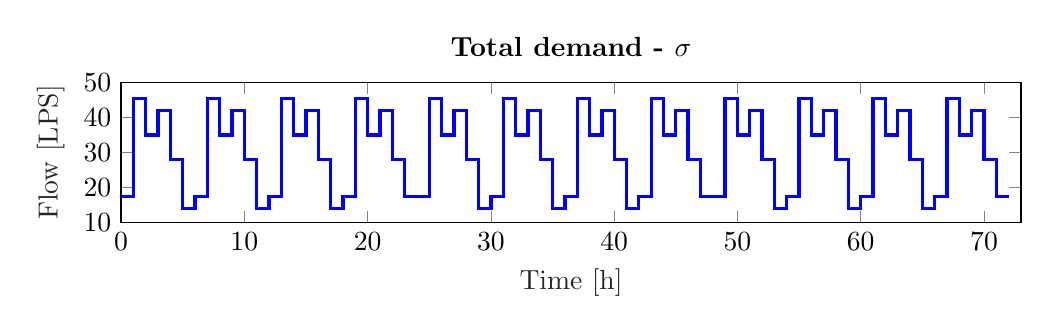
\begin{tikzpicture}

\begin{axis}[%
width=4.5in,
height=0.7in,
at={(0.784in,0.435in)},
scale only axis,
xmin=0,
xmax=73,
xlabel style={font=\color{white!15!black}},
xlabel={Time [h]},
ymin=10,
ymax=50,
ylabel style={font=\color{white!15!black}},
ylabel={Flow  [LPS]},
axis background/.style={fill=white},
title style={font=\bfseries},
title={Total demand - $\sigma$}
]
\addplot[const plot, color=blue, line width=1.2pt, forget plot] table[row sep=crcr] {%
0	17.5\\
1	45.5\\
2	35\\
3	42\\
4	28\\
5	14\\
6	17.5\\
7	45.5\\
8	35\\
9	42\\
10	28\\
11	14\\
12	17.5\\
13	45.5\\
14	35\\
15	42\\
16	28\\
17	14\\
18	17.5\\
19	45.5\\
20	35\\
21	42\\
22	28\\
23	17.5\\
24	17.5\\
25	45.5\\
26	35\\
27	42\\
28	28\\
29	14\\
30	17.5\\
31	45.5\\
32	35\\
33	42\\
34	28\\
35	14\\
36	17.5\\
37	45.5\\
38	35\\
39	42\\
40	28\\
41	14\\
42	17.5\\
43	45.5\\
44	35\\
45	42\\
46	28\\
47	17.5\\
48	17.5\\
49	45.5\\
50	35\\
51	42\\
52	28\\
53	14\\
54	17.5\\
55	45.5\\
56	35\\
57	42\\
58	28\\
59	14\\
60	17.5\\
61	45.5\\
62	35\\
63	42\\
64	28\\
65	14\\
66	17.5\\
67	45.5\\
68	35\\
69	42\\
70	28\\
71	17.5\\
72	17.5\\
};
\end{axis}
\end{tikzpicture}% 
 \vspace{-1.5mm}
 \caption{Total demand in the network.}
 \label{fig:sigma_example}
 \end{figure}

   %Inlet pressures
 \begin{figure}[H]
 \centering
 %
\includegraphics[width=0.35\textwidth]{report/pictures/missingfigure}
 % This file was created by matlab2tikz.
%
%The latest updates can be retrieved from
%  http://www.mathworks.com/matlabcentral/fileexchange/22022-matlab2tikz-matlab2tikz
%where you can also make suggestions and rate matlab2tikz.
%
\definecolor{mycolor1}{rgb}{0.00000,0.44700,0.74100}%
%
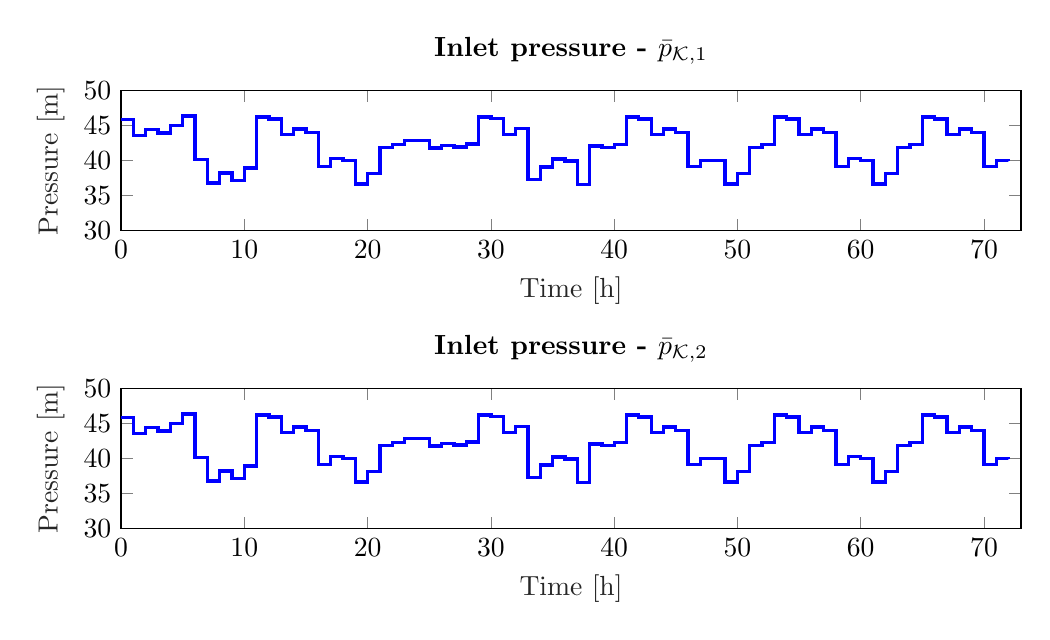
\begin{tikzpicture}

\begin{axis}[%
width=4.5in,
height=0.7in,
at={(0.892in,1.998in)},
scale only axis,
xmin=0,
xmax=73,
xlabel style={font=\color{white!15!black}},
xlabel={Time [h]},
ymin=30,
ymax=50,
ylabel style={font=\color{white!15!black}},
ylabel={Pressure  [m]},
axis background/.style={fill=white},
title style={font=\bfseries},
title={Inlet pressure - $\bar{p}_{\mathcal{K},1}$}
]
\addplot[const plot, color=blue, line width=1.2pt, forget plot] table[row sep=crcr] {%
0	45.8311\\
1	43.6012\\
2	44.3888\\
3	43.9077\\
4	45.035\\
5	46.3319\\
6	40.1154\\
7	36.7658\\
8	38.2118\\
9	37.1648\\
10	38.9031\\
11	46.1904\\
12	45.9122\\
13	43.6984\\
14	44.4791\\
15	44.0025\\
16	39.116\\
17	40.2569\\
18	39.9946\\
19	36.645\\
20	38.091\\
21	41.8587\\
22	42.3105\\
23	42.8635\\
24	42.8895\\
25	41.7857\\
26	42.1098\\
27	41.9096\\
28	42.36\\
29	46.2228\\
30	45.9453\\
31	43.7381\\
32	44.516\\
33	37.3111\\
34	39.0495\\
35	40.1904\\
36	39.928\\
37	36.5784\\
38	42.0576\\
39	41.8578\\
40	42.3096\\
41	46.1898\\
42	45.9116\\
43	43.6977\\
44	44.4785\\
45	44.0019\\
46	39.1175\\
47	40.0217\\
48	39.9897\\
49	36.64\\
50	38.0861\\
51	41.8589\\
52	42.3107\\
53	46.1905\\
54	45.9123\\
55	43.6986\\
56	44.4793\\
57	44.0027\\
58	39.1157\\
59	40.2566\\
60	39.9942\\
61	36.6446\\
62	38.0907\\
63	41.8587\\
64	42.3105\\
65	46.1904\\
66	45.9122\\
67	43.6984\\
68	44.4791\\
69	44.0025\\
70	39.1161\\
71	40.0203\\
72	39.9882\\
};
\end{axis}

\begin{axis}[%
width=4.5in,
height=0.7in,
at={(0.892in,0.508in)},
scale only axis,
xmin=0,
xmax=73,
xlabel style={font=\color{white!15!black}},
xlabel={Time [h]},
ymin=30,
ymax=50,
ylabel style={font=\color{white!15!black}},
ylabel={Pressure  [m]},
axis background/.style={fill=white},
title style={font=\bfseries},
title={Inlet pressure - $\bar{p}_{\mathcal{K},2}$}
]
\addplot[const plot, color=blue, line width=1.2pt, forget plot] table[row sep=crcr] {%
0	45.8311\\
1	43.6012\\
2	44.3888\\
3	43.9077\\
4	45.035\\
5	46.3319\\
6	40.1154\\
7	36.7658\\
8	38.2118\\
9	37.1648\\
10	38.9031\\
11	46.1904\\
12	45.9122\\
13	43.6984\\
14	44.4791\\
15	44.0025\\
16	39.116\\
17	40.2569\\
18	39.9946\\
19	36.645\\
20	38.091\\
21	41.8587\\
22	42.3105\\
23	42.8635\\
24	42.8895\\
25	41.7857\\
26	42.1098\\
27	41.9096\\
28	42.36\\
29	46.2228\\
30	45.9453\\
31	43.7381\\
32	44.516\\
33	37.3111\\
34	39.0495\\
35	40.1904\\
36	39.928\\
37	36.5784\\
38	42.0576\\
39	41.8578\\
40	42.3096\\
41	46.1898\\
42	45.9116\\
43	43.6977\\
44	44.4785\\
45	44.0019\\
46	39.1175\\
47	40.0217\\
48	39.9897\\
49	36.64\\
50	38.0861\\
51	41.8589\\
52	42.3107\\
53	46.1905\\
54	45.9123\\
55	43.6986\\
56	44.4793\\
57	44.0027\\
58	39.1157\\
59	40.2566\\
60	39.9942\\
61	36.6446\\
62	38.0907\\
63	41.8587\\
64	42.3105\\
65	46.1904\\
66	45.9122\\
67	43.6984\\
68	44.4791\\
69	44.0025\\
70	39.1161\\
71	40.0203\\
72	39.9882\\
};
\end{axis}
\end{tikzpicture}% 
 \vspace{-1.5mm}
 \caption{Inlet pressuresof the two pumping stations PU1 and PU2.}
 \label{fig:sigma_example}
 \end{figure}

\section{Validation tests}
\label{validation_tests} 

abcd

\chapter{Example network description}
\label{physical_properties_example1}

\emph{In this part of the appendix, the corresponding physical parameters of the Multi-inlet, Single-WT example network are given.}




